\section{Decoherence and Social-Graph Cascade}
\label{sec:cascade}

A projective poke isolates its consequences only when partners remain socially
disconnected. Whenever partners share mutual friends, institutions, or digital
group chats, information triggered by one partner's poke propagates across the
network, converting a local inquiry into system-wide \emph{decoherence}.

\subsection{The Social-Graph Model}
\label{subsec:cas-graph}

Let $G_{\mathrm{soc}} = (V, E)$ be an undirected simple graph~\citep{diestel2017graph,bollobas1998modern}
with vertex set $V = \partnerset = \{G_1, \dots, G_n\}$ representing the active
partners and edge set $E \subseteq \binom{V}{2}$ representing communication
channels (direct acquaintance, shared friend circles, or overlapping group
chats) through which two partners can compare notes.

When partner $G_{i_0}$ experiences or initiates a poke, he enters the
\emph{informed/comparing} state. Along each incident social edge $\{u, v\} \in E$,
an informed partner $u$ shares status observations with $v$ independently with
transmission probability $p_{\mathrm{tx}} \in (0, 1]$, reflecting conversational
proximity and willingness to compare timelines. Deleting each edge of
$G_{\mathrm{soc}}$ independently with probability $1 - p_{\mathrm{tx}}$ yields
the effective \emph{open-transmission subgraph} $G_{\mathrm{open}}$.

\begin{figure}[htbp]
  \centering
  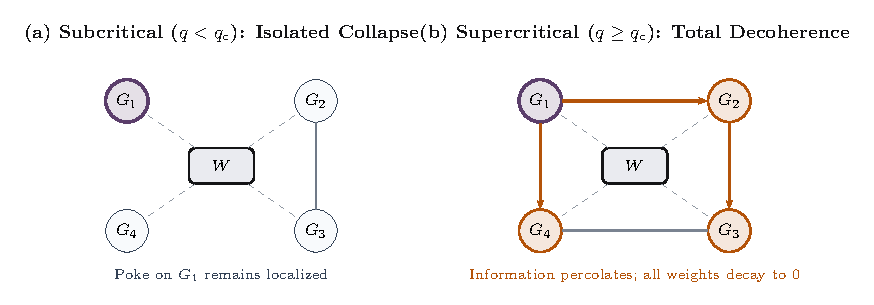
\includegraphics[width=0.95\textwidth]{figures/fig_social_graph.pdf}
  \caption{Social-graph decoherence regimes. (a) Subcritical graph ($q < q_c$):
  sparse links isolate a poke on $G_1$. (b) Supercritical graph ($q \ge q_c$):
  note-sharing percolates across connected partners, collapsing all active
  amplitudes toward zero.}
  \label{fig:social-graph}
\end{figure}

\subsection{Threshold Cascade and Percolation Transition}
\label{subsec:cas-percolation}

\begin{definition}[Decoherence cascade]
\label{def:cascade}
Let $C(i_0) \subseteq V$ denote the connected component of the initial poked
partner $i_0$ in the open-transmission subgraph $G_{\mathrm{open}}$. For a
critical awareness fraction $\theta \in (0, 1]$ (for instance, $\theta = 0.60$),
a \emph{decoherence cascade} occurs if
\begin{equation}
  \frac{\abs{C(i_0)}}{n} \;\ge\; \theta,
  \label{eq:cascade-condition}
\end{equation}
in which case cross-partner verification destroys relational coherence and
forces all active amplitudes $a_i \to 0$.
\end{definition}

In a homogeneous random graph~\citep{bollobas1998modern,grimmett1999percolation}
where each pair $\{i, j\}$ shares a social tie independently with edge density
$q \in [0, 1]$, each pair is linked by an open transmission edge with effective
bond probability $q_{\mathrm{eff}} = q\,p_{\mathrm{tx}}$. The expected number of
secondary partners alerted directly by a single newly informed partner (ignoring
boundary saturation) is therefore $(n - 1)\,q\,p_{\mathrm{tx}}$.

\begin{theorem}[Percolation threshold and fragility scaling]
\label{thm:percolation-threshold}
In the homogeneous social graph on $n \ge 2$ partners with edge density $q$ and
transmission probability $p_{\mathrm{tx}} > 0$:
\begin{enumerate}[nosep]
  \item the branching-process criticality condition $(n - 1) q p_{\mathrm{tx}} = 1$
        defines the critical edge density
        \begin{equation}
          q_c = \frac{1}{(n - 1)\,p_{\mathrm{tx}}};
          \label{eq:q-crit}
        \end{equation}
  \item for $q < q_c$, the expected size of the informed cluster starting from
        a single poked partner is bounded by the subcritical geometric series
        $\E[\abs{C(i_0)}] \le \bigl(1 - (n - 1) q p_{\mathrm{tx}}\bigr)^{-1}$,
        so large-$n$ cascades are exponentially suppressed;
  \item for $q > q_c$, an $O(n)$ giant informed component emerges, and the
        probability of cascade increases monotonically with both $q$ and the
        number of connected partners.
\end{enumerate}
\end{theorem}
\begin{proof}
Explore $C(i_0)$ via breadth-first search starting from $i_0$. At each step, an
unvisited vertex is reached across an open edge with probability $q p_{\mathrm{tx}}$.
Dominating the exploration by a Galton-Watson branching process with offspring
distribution $\operatorname{Binomial}(n - 1, q p_{\mathrm{tx}})$ gives mean
offspring $\mu = (n - 1) q p_{\mathrm{tx}}$~\citep{grimmett1999percolation,bollobas1998modern}.
When $\mu < 1$, i.e., $q < q_c$, total progeny has finite expectation
$(1 - \mu)^{-1}$, establishing (2). When $\mu > 1$, the survival probability of
the branching process is strictly positive, driving macroscopic percolation across
a constant fraction of vertices, while edge-coupling monotonicity~\citep{grimmett1999percolation}
guarantees that adding shared-friend edges or partners never decreases
$\Prob(\abs{C(i_0)} \ge \theta n)$, establishing (3) and proving \cref{prop:fragility}.
\end{proof}

\begin{proposition}[Fragility under shared social circles]
\label{prop:fragility}
The probability of total decoherence cascade is nondecreasing in the number of
partners who share edges in $G_{\mathrm{soc}}$.
\end{proposition}

\subsection{Effect of Network Topology: Homogeneous, Clustered, and Hub-Mediated}
\label{subsec:cas-topology}

Real social circles rarely match uniform random graphs; two structured
topologies arise frequently in practice~\citep{watts2002simple,granovetter1978threshold}:
\begin{itemize}[nosep]
  \item \textbf{Clustered circles.} Partners fall into two semi-isolated friend
        groups (e.g., workplace vs university), with high intra-circle density
        and sparse cross-circle bridges. Cascades easily wipe out an entire
        circle below $q_c$, while global collapse waits on the first bridge edge.
  \item \textbf{Hub-mediated networks.} One highly social partner acts as a
        central hub connected to many others. If the hub is poked or reached
        early, cascade probability spikes even at low global edge density;
        conversely, if peripheral partners lack ties to one another, isolation
        of the hub protects the system.
\end{itemize}

\begin{figure}[htbp]
  \centering
  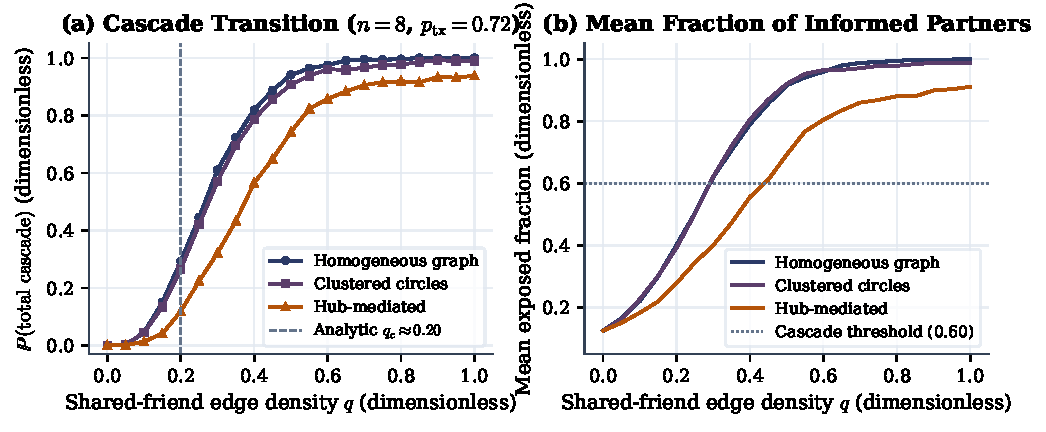
\includegraphics[width=0.95\textwidth]{figures/fig_cascade_percolation.pdf}
  \caption[Synthetic social-graph percolation curves across topologies]{Synthetic Monte Carlo percolation curves across $n = 8$ partners,
  $p_{\mathrm{tx}} = 0.72$, and $\theta = 0.60$ (\texttt{scripts/run\_simulations.py},
  seed \texttt{202603}, $1{,}500$ trials per point). (a) Probability of total
  cascade vs edge density $q$, showing the analytic threshold $q_c \approx 0.198$.
  (b) Mean fraction of informed partners.}
  \label{fig:cascade-percolation}
\end{figure}

In \cref{fig:cascade-percolation} (seed \texttt{202603}), the analytic
homogeneous threshold $q_c = \frac{1}{7 \times 0.72} \approx 0.1984$ aligns closely
with the onset of the steep transition: on homogeneous graphs, cascade
probability is $0.293$ at $q = 0.20$ and climbs to $0.975$ by $q = 0.60$.
Hub-mediated networks trigger cascades earlier at low density ($q \in [0.10, 0.25]$)
before saturating slightly more slowly due to disconnected peripheral pairs.

\subsection{Exact Combinatorial Cascade Polynomials for Small \texorpdfstring{$n$}{n}}
\label{subsec:cas-small-n}

While \cref{thm:percolation-threshold} describes asymptotic branching behavior
at moderate or large $n$, many real situationships operate with $n \in \{3, 4, 5\}$
partners, where every subgraph of $K_n$ can be enumerated explicitly as a
polynomial in the effective bond probability $q_{\mathrm{eff}} = q\,p_{\mathrm{tx}}$.
Under threshold $\theta = 0.60$, a cascade requires $\abs{C(i_0)} \ge \lceil 0.60 n \rceil$:
\begin{itemize}[nosep]
  \item For $n = 3$ ($\abs{C(i_0)} \ge 2$), a cascade fails only if the initial
        poked vertex has degree~$0$ in $G_{\mathrm{open}}$, giving
        \begin{equation*}
          P_{\mathrm{cas}}(3; q_{\mathrm{eff}}) = 1 - (1 - q_{\mathrm{eff}})^2 = 2q_{\mathrm{eff}} - q_{\mathrm{eff}}^2.
        \end{equation*}
  \item For $n = 4$ ($\abs{C(i_0)} \ge 3$), exact enumeration over all $2^6 = 64$
        labeled subgraphs of $K_4$ yields
        \begin{equation*}
          P_{\mathrm{cas}}(4; q_{\mathrm{eff}}) = 9q_{\mathrm{eff}}^2 - 17q_{\mathrm{eff}}^3 + 12q_{\mathrm{eff}}^4 - 3q_{\mathrm{eff}}^5.
        \end{equation*}
  \item For $n = 5$ ($\abs{C(i_0)} \ge 3$), enumeration over all $2^{10} = 1{,}024$
        subgraphs of $K_5$ yields
        \begin{equation*}
          P_{\mathrm{cas}}(5; q_{\mathrm{eff}}) = 18q_{\mathrm{eff}}^2 - 56q_{\mathrm{eff}}^3 + 79q_{\mathrm{eff}}^4 - 60q_{\mathrm{eff}}^5 + 24q_{\mathrm{eff}}^6 - 4q_{\mathrm{eff}}^7.
        \end{equation*}
\end{itemize}
For example, at $q = 0.30$ and $p_{\mathrm{tx}} = 0.72$ ($q_{\mathrm{eff}} = 0.216$),
exact evaluation gives $P_{\mathrm{cas}}(4; 0.216) = 0.2733$ and
$P_{\mathrm{cas}}(5; 0.216) = 0.4216$, illustrating how adding even a single
shared-circle partner sharply increases small-portfolio fragility.
